%*****************************************
\chapter{Der Soziale Netzwerke Vergleich}\label{ch:vergleich}
%*****************************************

Im vorherigen Teil der Arbeit haben wir uns damit beschäftigt, wie soziale Netzwerke so gut und realitätsnah wie möglich konstruiert werden können. Wir haben Analysen durchgeführt und festgestellt, dass die Werte unserer \textbf{Grad-} und \textbf{Nähe-Zentralität} näherungsweise normalverteilt sind. Daher liegt es nahe, weitere sozialen Netzwerke und ihre Analysen zum Vergleich heranzuziehen. Leitfragen sind hierbei, was zu erwarten ist, ob die Ergebnisse den Erwartungen entsprechen oder sogar widersprechen und warum dies der Fall ist. Zusätzlich möchten wir optimalerweise eine Möglichkeit erarbeitet, wie wir unsere Graphen bzw. die Generierung angepasst könnten um möglicherweise noch bessere Graphen zu erhalten, die die sozialen Netzwerken noch mehr ähneln. 

\section{Der Datensatz und die Analyse}
Auf der Suche nach vergleichbaren sozialen Netzwerken, beziehungsweise Datensätzen, ist die Suche scheinbar endlos. Auf vielen Webseiten sind große Datensätze für alle Nutzer*innen zugänglich. Meistens als \textbf{CSV} Datei, welche ideal zur Erstellung von Graphen mit unserem Generator geeignet sind. In diesem Teil der Arbeit betrachten wir mehrere Datensätze. Natürlich aufgrund der Tatsache, dass sie spannend sind aber auch um mehrere Vergleichswerte zu haben. Starten wir zunächst mit den Daten \cite{GOT} von unserem \textbf{Game of Thrones} Plot \ref{fig:GameOfThrones}. Da bereits die Analyse der \textbf{Zentralitäten} und die generelle visuelle Analyse des Graphen durchgeführt ist, reicht nun lediglich die Verteilung der Zentralitäten zu betrachten. Die Tabelle mit den Werten der Zentralitätsberechnungen befinden sich erneut in \cite{TZ}. Nachdem der Datensatz als \textbf{CSV} Datei in dem Generator eingelesen und anschließend geplottet wurde, wird folgender Graph konstruiert:

\FloatBarrier
\begin{figure}[h!]%
  \centering
  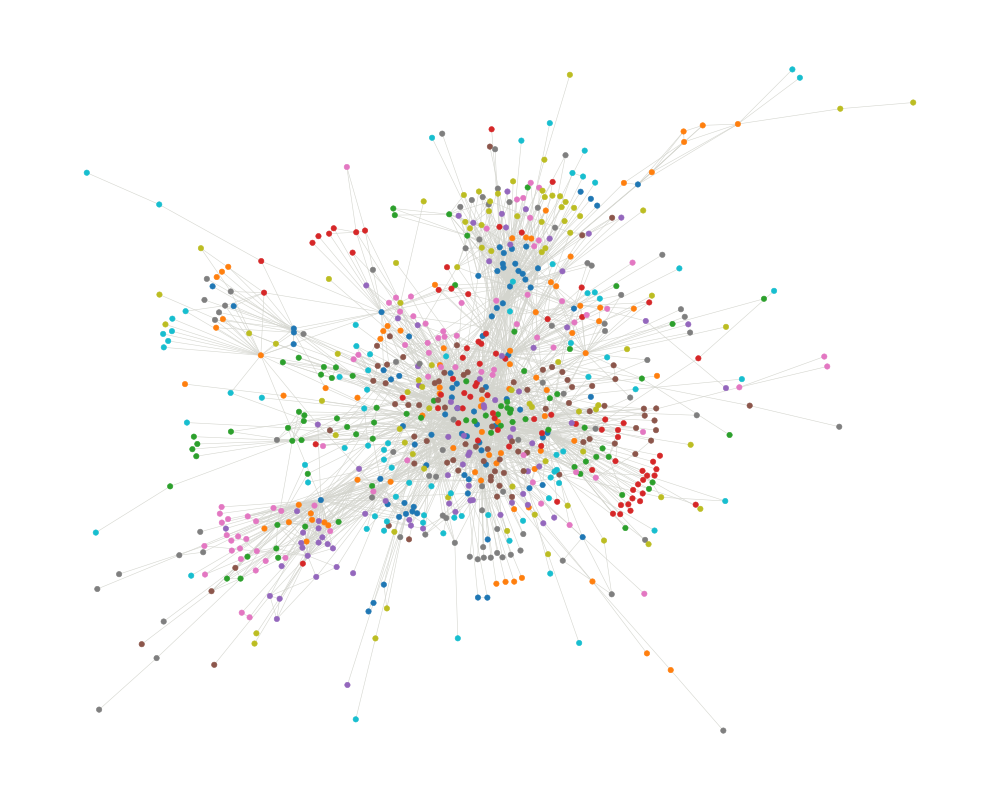
\includegraphics[width=0.7\textwidth]{Graphics/GOTPlot.png}
  \caption{Game of Thrones Graph 2.0, \\
  selbst erstellt}
  \label{fig:GOT2.0}
\end{figure}
\FloatBarrier

Dieser Plot bleibt beabsichtigt unkommentiert, da er lediglich zur Argumentation für die Verteilung der Zentralitäten benötigt wird und daher die visuelle Form des Graphen nur von zweitrangiger Bedeutung für diese Arbeit ist. Zudem ist zu vermerken, dass der eigentliche Datensatz gewichtet ist, und die bisher generierten Graph daher bereits schon visuell nicht dem Graphen aus \ref{fig:GameOfThrones} ähnelt. Jedoch ist es sinnvoll die Gewichte außen vor zu lassen, da in dieser Arbeit ausschließlich ungewichtete Graphen nachbildet beziehungsweise behandelt werden. Nachdem die Daten des Graphen \ref{fig:GOT2.0} eingelesen, die Zentralitäten berechnet sind und anschließend die Balkengraphen erstellt wurden, ist folgender Plot entstanden:

\FloatBarrier
\begin{figure}[h!]%
  \centering
   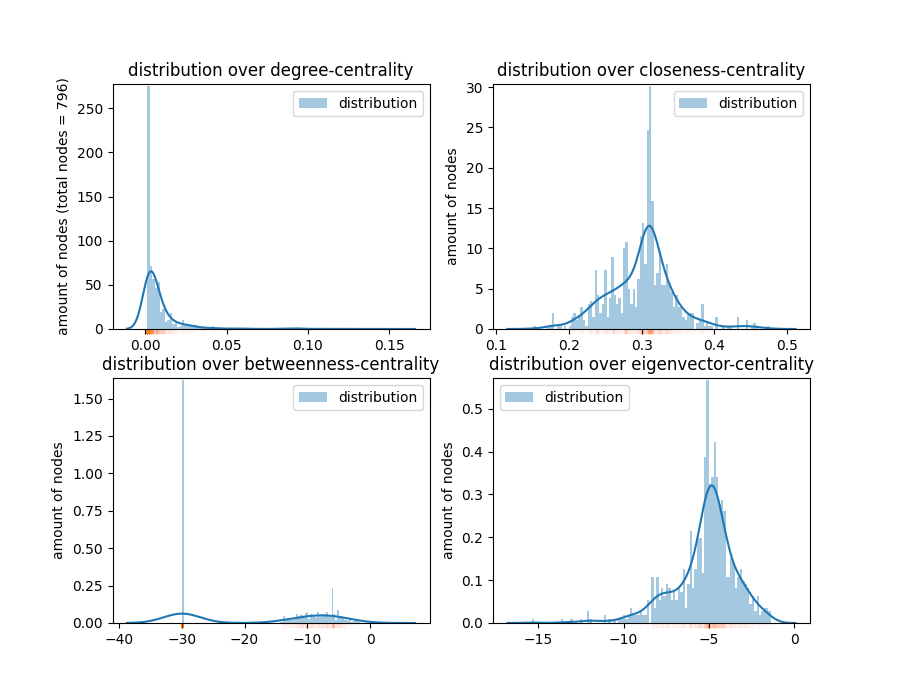
\includegraphics[width=0.8\textwidth]{Graphics/GOT-Distribution.png}
  \caption{Game of Thrones Verteilung der Zentralitäten}
  \label{fig:distributionGOT}
\end{figure}
\FloatBarrier
 
 Auf den ersten Blick wird bereits klar, dass andere Ergebnisse erwartet wurden. Einzig die Verteilung der \textbf{Nähe-Zentralität} ähnelt der erwarteten Normalverteilung. Die \textbf{Betweenness-} und \textbf{Eigenvektor-Zentralität} hingegen ähneln zwar nicht exakt dem, was in \ref{fig:distributionALL} herausgekommen ist, aber zieht auf jeden Fall Parallelen. Denn beide haben einen Ausschlag von mindestens einem Balken, was bereits im vorherigen Kapitel damit begründet wurde, dass es die Folge von vielen kürzesten Wegen ist, die stets über die gleichen
Knoten verlaufen. Daher keine Alternativen im Graph existieren. Die \textbf{Grad-Zentralität} hingegen ist tatsächlich verwunderlich. Sie ähnelt keinesfalls der Normalverteilung aber sieht sehr nach einer Exponentialverteilugn aus. Der Ausschlag der Balken ist hingegen schnell erklärt. Es sind viele Konten, in diesem Fall repräsentierte \textit{Game of Thrones} Charaktere, die alle gleich wichtig für den Graphen sind. Diese Knoten sind daher mit vielen anderen Knoten verbunden, werden also von vielen anderen Charakteren gekannt oder kennen viele andere Charaktere. Im Allgemeinen sind die Balkendiagramme der \textbf{Zentralitäten} aus \ref{fig:distributionGOT} leider nicht zufriedenstellend. Der Grund, warum die Ergebnisse stark von unseren Erwartungen abweicht ist vermutlich, dass es sich bei dem Graphen um fiktive Charaktere handelt. Dadurch kann es schnell zu Unstimmigkeiten kommen. Zudem war der Datensatz davor gewichtet, was zu anderen Werten bei der Berechnung der Zentralitäten führen kann. Doch wurde der Datensatz ungewichtet betrachtet, um ihn besser mit den generierten Graphen zu vergleichen, welche ungewichtet sind. Dies kann auf jeden Fall ein plausibler Grund für Unstimmigkeiten sein. Zudem haben ist die Anzahl der geplotteten Balken stark erhöht und so fallen Unstimmigkeiten generell deutlich schneller auf. Dennoch soll die Theorie, dass Zentralitäten normalverteilterteilt sind, nicht verworfen werden und wir betrachten noch einen weiteren Datensatz. Der nächste Datensatz, der aus aus "Kreisen" (oder "Freundeslisten") besteht, ist von Facebook veröffentlicht worden. Die Daten wurden jedoch vor der Veröffentlichung von Facebook anonymisiert, daher ist lediglich bekannt, dass es sich bei dem Datensatz um politische Interessen handelt. So kann mit dem Datensatz feststellt werden, dass zwei Nutzer die gleiche politische Zugehörigkeit haben, aber nicht, was ihre individuelle politische Zugehörigkeit bedeutet \cite{FBData}.
Nachdem die Daten wieder in eine \textbf{.CSV} Datei umgewandelt und anschließend geplottet wurden, ist folgenden Graphen entstanden: 


\FloatBarrier
\begin{figure}[h!]%
  \centering
 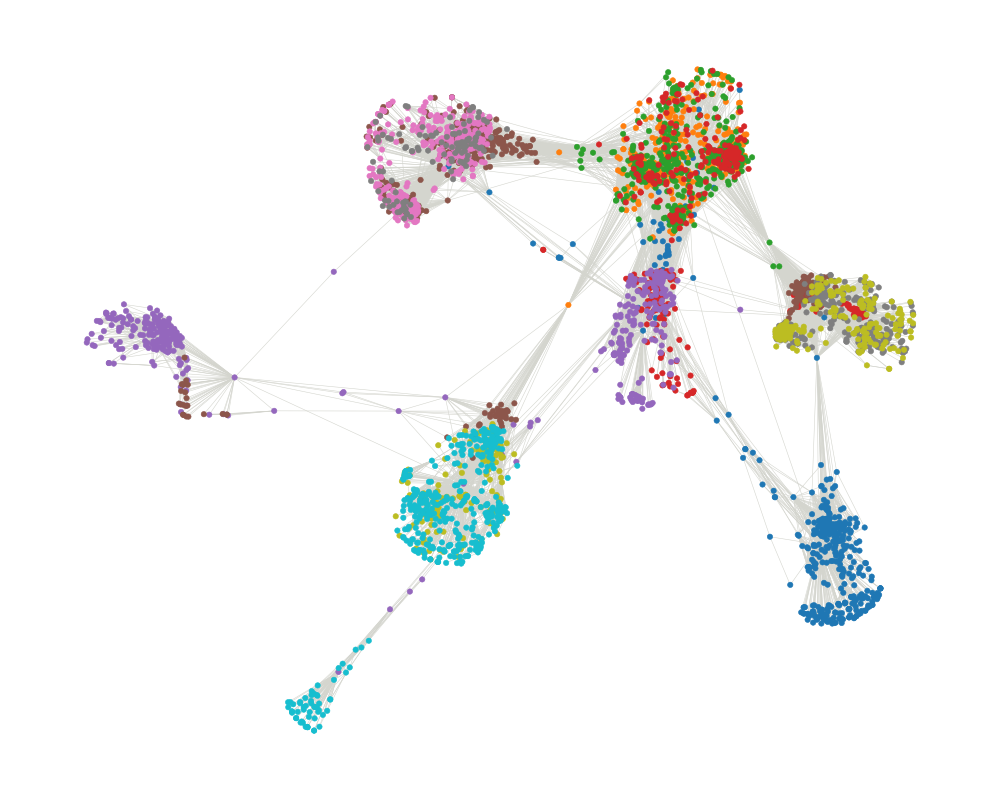
\includegraphics[width=0.7\textwidth]{Graphics/FacebookPoliticalPlot.png}
  \caption{Facebook Graph}
  \label{fig:FacebookGraph}
\end{figure}
\FloatBarrier



Der Graph ähnelt auf den ersten Blick keinem, der bisher generierten Graphen. Zudem fällt aber sofort auf, dass dieser Graph aus deutlich mehr Knoten besteht, zudem weniger Subgraphen besitzt aber dennoch eine grundsätzlich ähnliche Struktur zu unseren anderen Graphen aufweist. Die Berechnungen der Zentralitäten befinden sich ebenfalls auf Github \cite{TZ}, da es sich um zu viele Werte handelt. Nun interessiert uns jedoch, wie diese Zentralitäten verteilt sind und ob dieser Graph die erwarteten Verteilungen nachweist. Nachdem der Graphe \ref{fig:FacebookGraph} durch unsere Methode, welche die Plots über die Verteilungen erstellt, gelaufen ist, sind folgende Diagramme entstanden:

\FloatBarrier
\begin{figure}[h!]%
  \centering
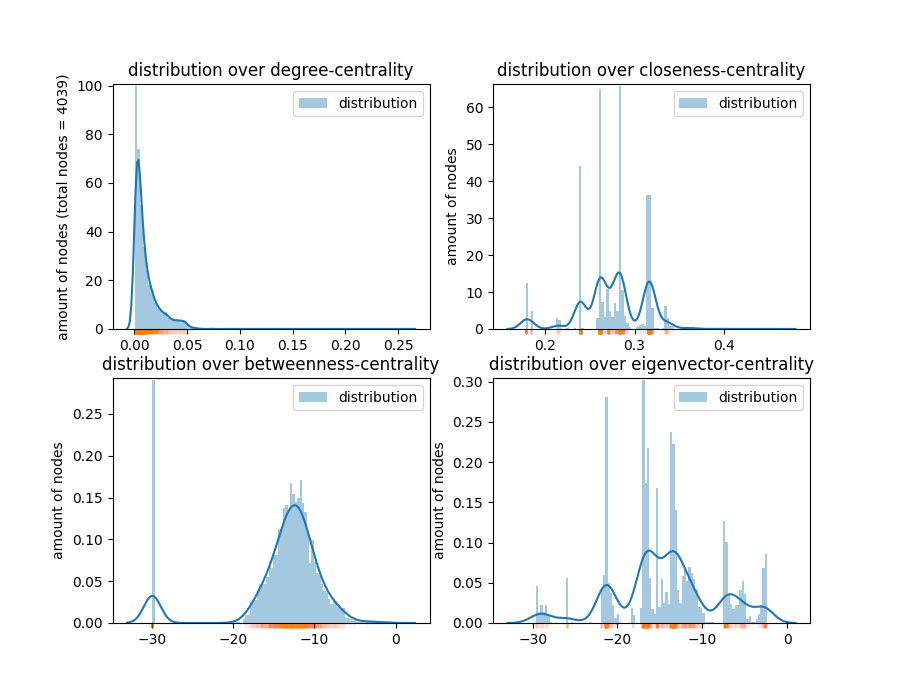
\includegraphics[width=0.8\textwidth]{Graphics/facebookLOG.png}
  \caption{Facebook Graph Distribution}
  \label{fig:FacebookGraphDistribution}
\end{figure}
\FloatBarrier

Sofort fällt auf, dass bei keiner Zentralität eine Normalverteilung erkennbar ist. Die \textbf{Grad-Zentralität} fällt aber direkt auf, denn es handelt sich hier um eine Exponentialverteilung. Die anderen Balkendiagramme der \textbf{Betweenness-} und \textbf{Eigenvektor-Zentralität} ähneln jedoch den Verteilungen aus \ref{fig:distributionALL}. Was zudem auffällig ist, dass die Diagramm stark an die Verteilungen von \ref{fig:distributionGOT} erinnern. Auch wenn diese Ergebnisse sehr ernüchtern scheinen und vor allem das Balkendiagramm der \textbf{Nähe-Zentralität} erneut nicht normalverteilt ist, wollen wir uns überlegen, woran dies liegen kann. Bei den anderen Zentarlitäten herrscht eine starke Fluktuation der Balken, wodurch keine Mathematischen Wahrscheinlichkeitsverteilungen erkennbar ist. Visuell fällt jedoch auf, dass der Graph \ref{fig:FacebookGraphDistribution} verglichen mit dem Plot des Graphen \ref{ch:SNA} durchaus Parallelen aufweist. Es sind aber deutliche Ansammlungen von Knoten, die auch als Teilgraphen bezeichnet werden können, ersichtlich. Zwischen den Teilgraphen sind, so wie bei \ref{fig:SNA}, einige Kanten zu erkennen, die Teilgraphen untereinander verbinden. Natürlich weist der obige Graph deutlich mehr Kanten und Knoten auf als die bisherigen Graphen. Unsere Graphen haben im Schnitt um die \textbf{950} Knoten und \textbf{8700} Kanten, daher also circa neun mal so viele Kanten wie Knoten. Auch existieren im Schnitt um die \textbf{10100} Cliquen, welche maximal acht Knoten groß sind. Bei dem Facebook Graphen \ref{fig:FacebookGraph} hingegen \textbf{4093} Knoten und \textbf{88234} Kanten. Das heißt circa einundzwanzig mal so viele Kanten wie Knoten. Leider ist die Anzahl an Knoten und Kanten des Graphen \ref{fig:FacebookGraph} nur durch die Homepage \cite{FBData} bekannt, denn der Datensatz ist leider zu groß, um die Analyse der Zentralitäten und die Untersuchung auf Cliquen zu Ende zu führen. Daher ist auch die genaue Anzahl an Cliquen dieses Graphen unbekannt, doch kann vermutet werden, dass diese sicherlich deutlich höher sind als bei \ref{fig:distributionALL}, denn es existieren mehr Knoten mit ähnlich hohen Zentralitäten. Schließlich wird noch ein letzter Versuch gestartet, die Kanten und Knoten im Code des Graphen Generators zu erhöhen, um damit die selbe Relation zu erhalten. Dadurch wird womöglich gezeigt, dass alle vier untersuchten Zentralitäten annähern Normalverteilt sind. Was zum einen daran liegt, dass letztendlich Graphen wie \ref{fig:GOT2.0} erhalten sind, die noch viel dichter besetzt sind und leider alle Knoten mit beinahe allen anderen Knoten verbunden sind, was eher untypisch für \textit{soziale Netzwerke} ist. Es darf aber auf jeden Fall festgehalten werden, dass die \textbf{Betweenness-} und \textbf{Eigenvektor-Zentralität} bei allen untersuchten Datensätzen starke Parallelen zu den Verteilungen des generierten sozialen Netzwerk nachweisen. Jedoch ist nach wie vor die Verteilung der \textbf{Gradzentralität} verwunderlich. Daher ist es ratsam, den Code und die damit verbundenen Plot so anzupassen, dass es dem Plot \ref{fig:FacebookGraphDistribution} ähnelt. Anschließend kann die Verteilungen der Zentralitäten betrachtet und dadurch eine genauere Aussage erzielt werden. 


\section{Anpassung des generierten Plots}
Nachdem die Verteilungen durchaus verwunderlich ist, wird der nächsten Plot weitestgehend an \ref{fig:FacebookGraphDistribution} angepasst. An dieser Stelle muss durchaus betont werden, dass es sich bei den bisher generierten Plot keinesfalls um untypische oder falsche soziale Netzwerke handelt. In diesem Abschnitt wird lediglich eine bessere Vergleichsbasis hergestellt. Dies wird ermöglicht, indem zum einen die Anzahl an Cluster auf \textbf{sieben} Stück anpasst und die Anzahl der Knoten pro Cluster erhöht wird. Gleichzeitig aber die jeweiligen Größen deutlich mehr variieren lassen und vor allem die Kanten-Menge, also Anzahl an Verbindungen, deutlich erhöhen. Schließlich erhält man folgende Graphen: 

\FloatBarrier
\begin{figure}[h!]%
  \centering
  \subfloat[][]{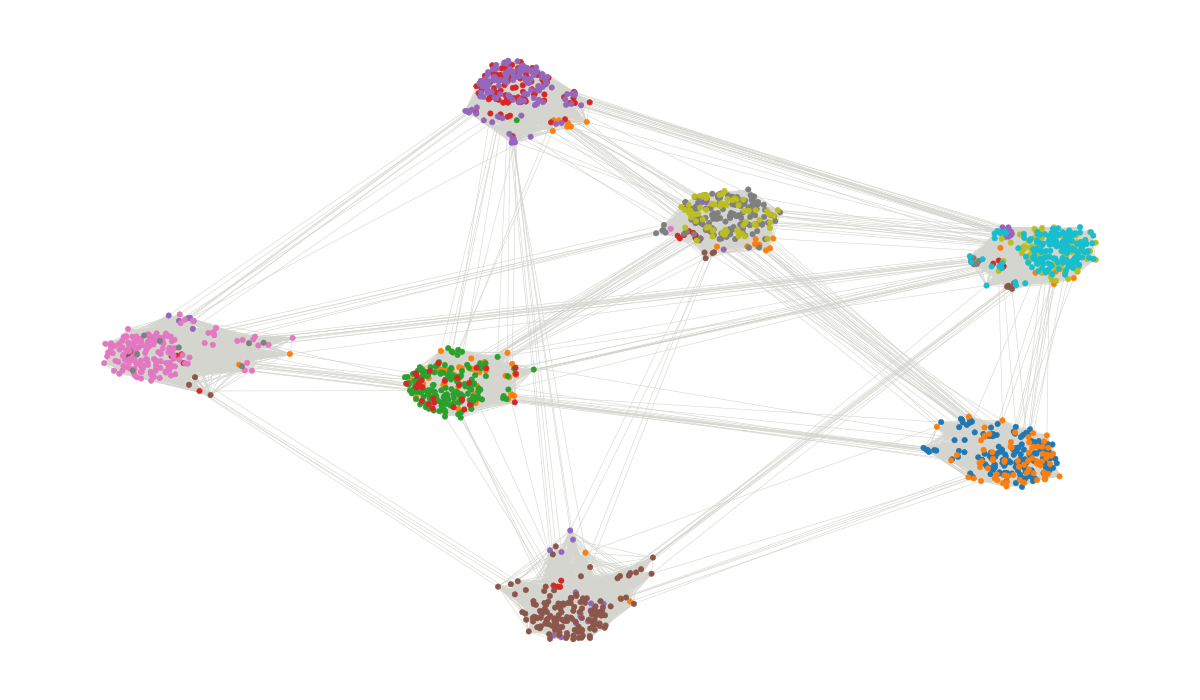
\includegraphics[width=0.8\textwidth]{Graphics/generatedPlotFinal.png}}%
  \qquad
  \subfloat[][]{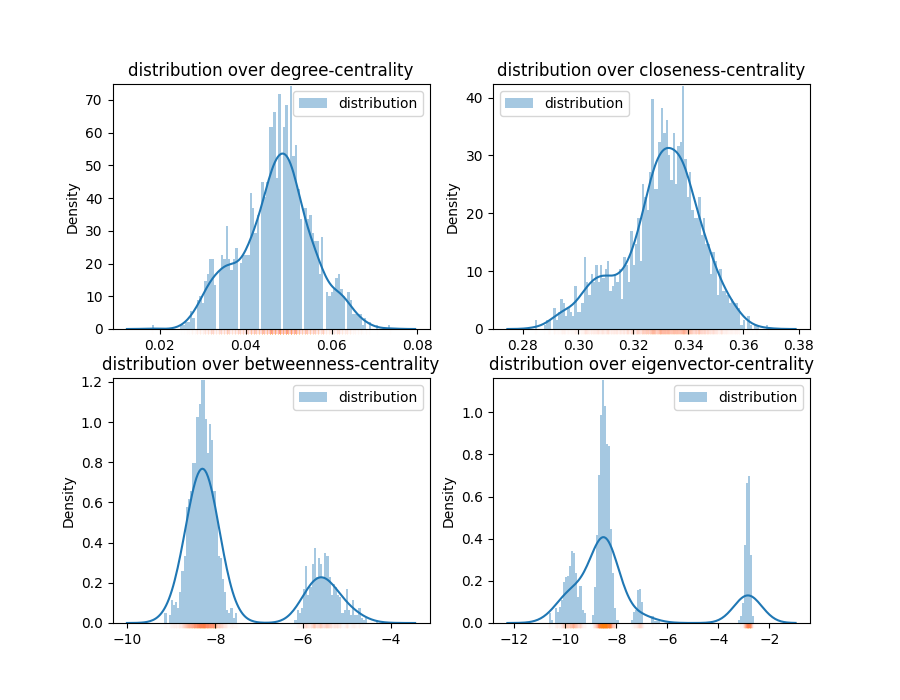
\includegraphics[width=0.7\textwidth]{Graphics/generatedPlotDensity.png}}
  \caption{Final optimierter Graph}
  \label{fig:ourGraphFinalPlot}
\end{figure}
\FloatBarrier

Natürlich ist direkt ersichtlich, ohne die Werte genauer analysiert zu haben, dass keine zu \ref{fig:FacebookGraphDistribution} identischen Graphen erzeugt werden können. Dies liegt an mehreren Faktoren, die unter anderem im Ausblick erörtern werden. Allgemein sind die, in dieser Arbeit generierten Graphen, auch wenn die Varianz der Graph-Größen best möglichst garantiert wird, auf den ersten Blick ähnlich groß. Jedoch wurde bei der Verteilung der Zwischen- und Eigenvektor Zentralität eine absolute Verbesserung erzielt, indem die Zentralitäten, bevor sie geplottet werden, logarithmiert werden. Dies wurde nachträglich auch bei allen vorherigen Verteilungen gemacht. Das ermöglicht es, die Verteilung auseinander zu zerren, da sich die Werte stets um \textbf{0.0} verteilt haben. Nun fällt auf, dass die Verteilungen dieser zwei Zentralitäten sehr ähnlich sind. Eine mögliche Begründung hierfür kann sein, dass die Eigenwert-Zentralität im Nachhinein betrachtet nicht sonderlich interessant ist. Nehmen wir an, dass \textit{$x^*$} ein nicht negativer Eigenvektor ist, mit einem Eintrag für jeden Knoten. Aufsummiert soll dieser \textit{1} ergeben. Dadurch darf er als Wahrscheinlichkeitsverteilung interpretiert werden. Für einen Knoten \textit{v} kann der Eintrag von \textit{$x^*_v$} als Eintrag seiner \textit{Eigenwert-Zentralität} gesehen werden. Tatsächlich kann ein Eigenvektor mit Bezug auf 1 leicht erraten werden. \\
Sein nun 
\begin{equation}
     x^*_v &= \frac{k_v}{2 \times |E|} \forall v \in V
     \label{proof}
\end{equation}
Wobei \textit{$k_v$} die \textit{Grad-Zentralität} des Knoten \textbf{v} ist und |E| die Anzahl an Kanten. Es folgt direkt, dass $x^*_v$ die Bedingungen für $x^*$ erfüllt. Tatsächlich erinnert uns \ref{proof} an \ref{degree} das heißt, die \textit{Eigenvektor-Zentralität} entspricht der mit einer Konstanten skalierten \textit{Grad-Zentralität}.
Das ist jedoch nur eine Vermutung und wird nicht mehr weiter betrachtet. Schließlich fehlt noch die Einordnung des \ref{fig:ourGraphFinalPlot} und \ref{fig:FacebookGraphDistribution}
Hier sind leider keine identischen Verteilungen entstanden. Tatsächlich kann dies auch mathematisch begründet werden, denn wenn zwei Zufallsvariablen \textbf{X} und \textbf{Y} standardnormalverteilt und unabhängig sind, dann wären für Parameter $\lambda = \frac{1}{2}$ die Variablen $X^2+Y^2$ exponentialverteilt \cite{verteilung}. Doch hat die Optimierung in diesem Kapitel dennoch viel gebracht. Unter anderem konnte bewiesen werden, dass mit wenigen Anpassungen des Codes, annähernd vergleichbare Verteilungen erhalten werden. Um den idealen Vergleich herzustellen, müssen jedoch größere Änderungen am Code vorgenommen werden, was jedoch nicht mehr im Umfang dieser Arbeit liegt. 



